\documentclass{standalone}
\usepackage{tikz}
\usepackage{ctex,siunitx,upgreek}
\setCJKmainfont{Noto Serif CJK SC}
\usepackage{tkz-euclide}
\usepackage{amsmath,amsfonts,amssymb}
\usetikzlibrary{patterns, calc,3d}
\usetikzlibrary {decorations.pathmorphing,decorations.pathreplacing,decorations.shapes}
\tikzset{label style/.append style={font=\small}}
\begin{document}
\small
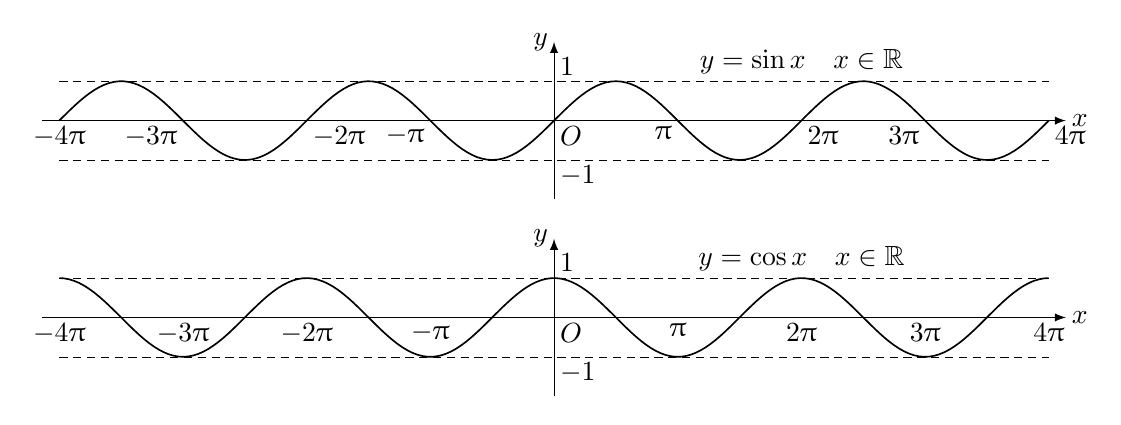
\begin{tikzpicture}[>=latex,scale=0.5,inner sep=2pt]
  \begin{scope}
    \draw[->](-13,0)--(13,0)node[right]{$x$};
    \draw[->](0,-2)--(0,2)node[left]{$y$};
    \node at (0,0)[below right]{$O$};
    \draw[semithick,samples=200,domain=-4*pi:4*pi]plot(\x,{sin(\x r)});
    \draw[densely dashed,very thin](-4*pi,1)--(4*pi,1);
    \draw[densely dashed,very thin](-4*pi,-1)--(4*pi,-1);
    \node at (2*pi,1.5){$y=\sin x\quad x\in\mathbb{R}$};
    \node at (-4*pi,0)[below]{$-4\uppi$};
    \node at (-3*pi,0)[below left]{$-3\uppi$};
    \node at (-2*pi,0)[below right]{$-2\uppi$};
    \node at (-pi,0)[below left]{$-\uppi$};
    \node at (pi,0)[below left]{$\uppi$};
    \node at (2*pi,0)[below right]{$2\uppi$};
    \node at (3*pi,0)[below left]{$3\uppi$};
    \node at (4*pi,0)[below right]{$4\uppi$};
    \node at (0,1)[above right]{1};
    \node at (0,-1)[below right]{$-1$};
  \end{scope}
  \begin{scope}[yshift=-5cm]
    \draw[->](-13,0)--(13,0)node[right]{$x$};
    \draw[->](0,-2)--(0,2)node[left]{$y$};
    \node at (0,0)[below right]{$O$};
    \draw[semithick,samples=200,domain=-4*pi:4*pi]plot(\x,{cos(\x r)});
    \draw[densely dashed,very thin](-4*pi,1)--(4*pi,1);
    \draw[densely dashed,very thin](-4*pi,-1)--(4*pi,-1);
    \node at (2*pi,1.5){$y=\cos x\quad x\in\mathbb{R}$};
    \node at (-4*pi,0)[below]{$-4\uppi$};
    \node at (-3*pi,0)[below]{$-3\uppi$};
    \node at (-2*pi,0)[below]{$-2\uppi$};
    \node at (-pi,0)[below]{$-\uppi$};
    \node at (pi,0)[below]{$\uppi$};
    \node at (2*pi,0)[below]{$2\uppi$};
    \node at (3*pi,0)[below]{$3\uppi$};
    \node at (4*pi,0)[below]{$4\uppi$};
    \node at (0,1)[above right]{1};
    \node at (0,-1)[below right]{$-1$};
  \end{scope}
\end{tikzpicture}
\end{document}